%% LyX 1.6.5 created this file.  For more info, see http://www.lyx.org/.
%% Do not edit unless you really know what you are doing.
\documentclass[english,handout]{beamer}
\usepackage[T1]{fontenc}
\usepackage[latin9]{inputenc}
\setcounter{secnumdepth}{3}
\setcounter{tocdepth}{3}
\usepackage{amsmath}
\usepackage{graphicx}
\usepackage{amssymb}

\makeatletter
%%%%%%%%%%%%%%%%%%%%%%%%%%%%%% Textclass specific LaTeX commands.
 % this default might be overridden by plain title style
 \newcommand\makebeamertitle{\frame{\maketitle}}%
 \AtBeginDocument{
   \let\origtableofcontents=\tableofcontents
   \def\tableofcontents{\@ifnextchar[{\origtableofcontents}{\gobbletableofcontents}}
   \def\gobbletableofcontents#1{\origtableofcontents}
 }
 \makeatletter
 \long\def\lyxframe#1{\@lyxframe#1\@lyxframestop}%
 \def\@lyxframe{\@ifnextchar<{\@@lyxframe}{\@@lyxframe<*>}}%
 \def\@@lyxframe<#1>{\@ifnextchar[{\@@@lyxframe<#1>}{\@@@lyxframe<#1>[]}}
 \def\@@@lyxframe<#1>[{\@ifnextchar<{\@@@@@lyxframe<#1>[}{\@@@@lyxframe<#1>[<*>][}}
 \def\@@@@@lyxframe<#1>[#2]{\@ifnextchar[{\@@@@lyxframe<#1>[#2]}{\@@@@lyxframe<#1>[#2][]}}
 \long\def\@@@@lyxframe<#1>[#2][#3]#4\@lyxframestop#5\lyxframeend{%
   \frame<#1>[#2][#3]{\frametitle{#4}#5}}
 \makeatother
 \def\lyxframeend{} % In case there is a superfluous frame end

%%%%%%%%%%%%%%%%%%%%%%%%%%%%%% User specified LaTeX commands.
\usepackage{amsfonts}

\usetheme{Madrid}

\title[ALARIStatisticsCourse]{ALARIStatisticsCourse}\subtitle{PartII}\author[ClaudioOrtelli]{ClaudioOrtelli}\institute[USI]{Universit\`{a}dellaSvizzeraitaliana}\date[29/2010]{April2011}

\makeatother

\usepackage{babel}

\begin{document}

\lyxframeend{}\lyxframe{Functions of random variables}
\begin{itemize}
\item Let $X$ be a continous random variable with distribution function
$F_{X}$, $\Psi$ a function and \[
Y=\Psi(X).\]

\item Under regularity conditions on $\Psi$, $Y$ is a random variable! 
\item Continuity or stepwise continuity of $\Psi$ are sufficient conditions
for $Y$ to be a random variable. \end{itemize}
\begin{exampleblock}
{Example: Quadratic cost function.} 

Let $X$ denote a measurement error. We assume a quadratic cost function,
i.e. $Y=\Psi(X)=X^{2}$. The random variable $Y$ has a distribution
function $F_{Y}$ which depends on $F_{X}$ and $\Psi$.
\end{exampleblock}

\lyxframeend{}


\lyxframeend{}\lyxframe{Functions of random variables}
\begin{itemize}
\item To derive $F_{Y}$ simply compute the preimage of the event $C=(-\infty,y]$.
In fact by definition of $F_{Y}$\begin{eqnarray*}
F_{Y}(y) & = & P(Y\leq y)=P(Y\in C)\\
 & = & P(\Psi(X)\in C)\\
 & = & P(\Psi^{-1}(C))\\
 & = & P_{X}(B)\end{eqnarray*}
where the set $B$ is the preimage of $C$, i.e.\[
B=\Psi^{-1}(C)=\{x\in\mathbb{R\mid}\Psi(x)\in C\}.\]

\item The preimage function of $\Psi$ is a set function (the arguments
are subsets of \textrm{$\mathbb{R}$}) and is defined even if $\Psi$
is not one-to-one.
\end{itemize}

\lyxframeend{}


\lyxframeend{}\lyxframe{Functions of random variables}

\noindent \begin{center}
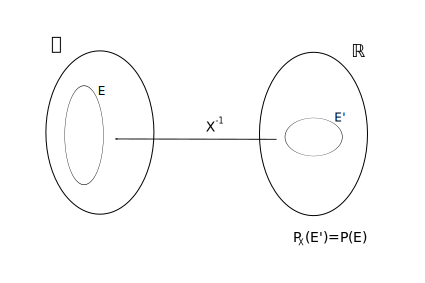
\includegraphics{codiceR/grafici/variabileAleatoria}
\par\end{center}


\lyxframeend{}\lyxframe{Functions of random variables}

\noindent \begin{center}
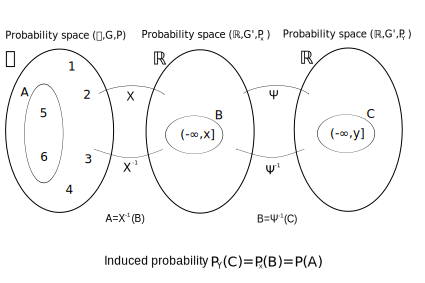
\includegraphics{codiceR/grafici/funzioneDivariabileAleatoria}
\par\end{center}


\lyxframeend{}
\lyxframe{Functions of random variables}
\begin{exampleblock}
{Example continued}

Because $Y=X^{2}\geqslant0$ and $X=\pm\sqrt{Y}$ 
\begin{itemize}
\item when $y\leq0$ it follows $F_{Y}(y)=0$;
\item when $y>0$ it follows $Y\leqslant y\Leftrightarrow-\sqrt{y}\leqslant X\leqslant\sqrt{y}$
so that $F_{Y}(y)=F_{X}(\sqrt{y})-F_{X}(-\sqrt{y})$.
\end{itemize}
\end{exampleblock}

\lyxframeend{}



\end{document}
